\chapter{Создание моделей}
\lstinputlisting[language=R,caption=, label=lst:models]{listings/models.R}

\begin{table}[h]
	\centering
	\caption{Сводная информация по первой модели: Drinks\_per\_week $\sim$ Party\_Hours\_per\_week + Gender}
	\begin{tabular}{lrrrr}
		\hline
		\textbf{Coefficient} & \textbf{Estimate} & \textbf{Std. Error} & \textbf{t value} & \textbf{Pr($>$$|$t$|$)} \\
		\hline
		(Intercept)             & 1.63 & 0.37 & 4.39  & 1.27e-06$^{***}$ \\
		Party\_Hours\_per\_week & 1.14 & 0.03 & 34.31 & $<$2e-16$^{***}$ \\
		Gender1                 & -2.25 & 0.39 & -5.73 & 1.34e-08$^{***}$ \\
		\hline
	\end{tabular}
	
	\vspace{0.5em}
	\textbf{Residuals:}\\
	Min: -46.40 \quad 1Q: -2.78 \quad Median: -0.511 \quad 3Q: 1.19 \quad Max: 43.36
	
	\vspace{0.5em}
	\textbf{Model Fit:}\\
	Residual standard error: 5.98 on 1019 degrees of freedom \\
	Multiple R-squared: 0.54 \quad Adjusted R-squared: 0.55 \\
	F-statistic: 614.3 on 2 and 1019 DF \quad p-value: $<$2.2e-16
		\label{tab:m1}
\end{table}

\begin{table}[h]
	\centering
	\caption{Сводная информация по второй модели: Drinks\_per\_week $\sim$ Party\_Hours\_per\_week + Gender + Home\_Town}
	\begin{tabular}{lrrrr}
		\hline
		\textbf{Coefficient} & \textbf{Estimate} & \textbf{Std. Error} & \textbf{t value} & \textbf{Pr($>$$|$t$|$)} \\
		\hline
		(Intercept)             & 1.85 & 0.45 & 4.09  & 4.56e-05$^{***}$ \\
		Party\_Hours\_per\_week & 1.15 & 0.03 & 34.28 & $<$2e-16$^{***}$ \\
		Gender1                 & -2.23 & 0.40 & -5.63 & 2.38e-08$^{***}$ \\
		Home\_Town              & -0.36 & 0.41 & -0.86 & 0.39 \\
		\hline
	\end{tabular}
	
	\vspace{0.5em}
	\textbf{Residuals:}\\
	Min: -46.351 \quad 1Q: -2.653 \quad Median: -0.420 \quad 3Q: 1.248 \quad Max: 48.499
	
	\vspace{0.5em}
	\textbf{Model Fit:}\\
	Residual standard error: 5.97 on 1018 degrees of freedom \\
	Multiple R-squared: 0.55 \quad Adjusted R-squared: 0.55 \\
	F-statistic: 409.7 on 3 and 1018 DF \quad p-value: $<$2.2e-16
	\label{tab:m2}
\end{table}

Сводная информация по созданным моделям приведена в таб. \ref{tab:m1} - \ref{tab:m2}.
Как можно видеть, добавление преобразованного города не является значимым. Но изменилась константа (Intercept).
\newpage
Построим графики обеих моделей (рис. \ref{fig:models}).
\begin{figure}[h]  % Окружение для картинки
	\centering
	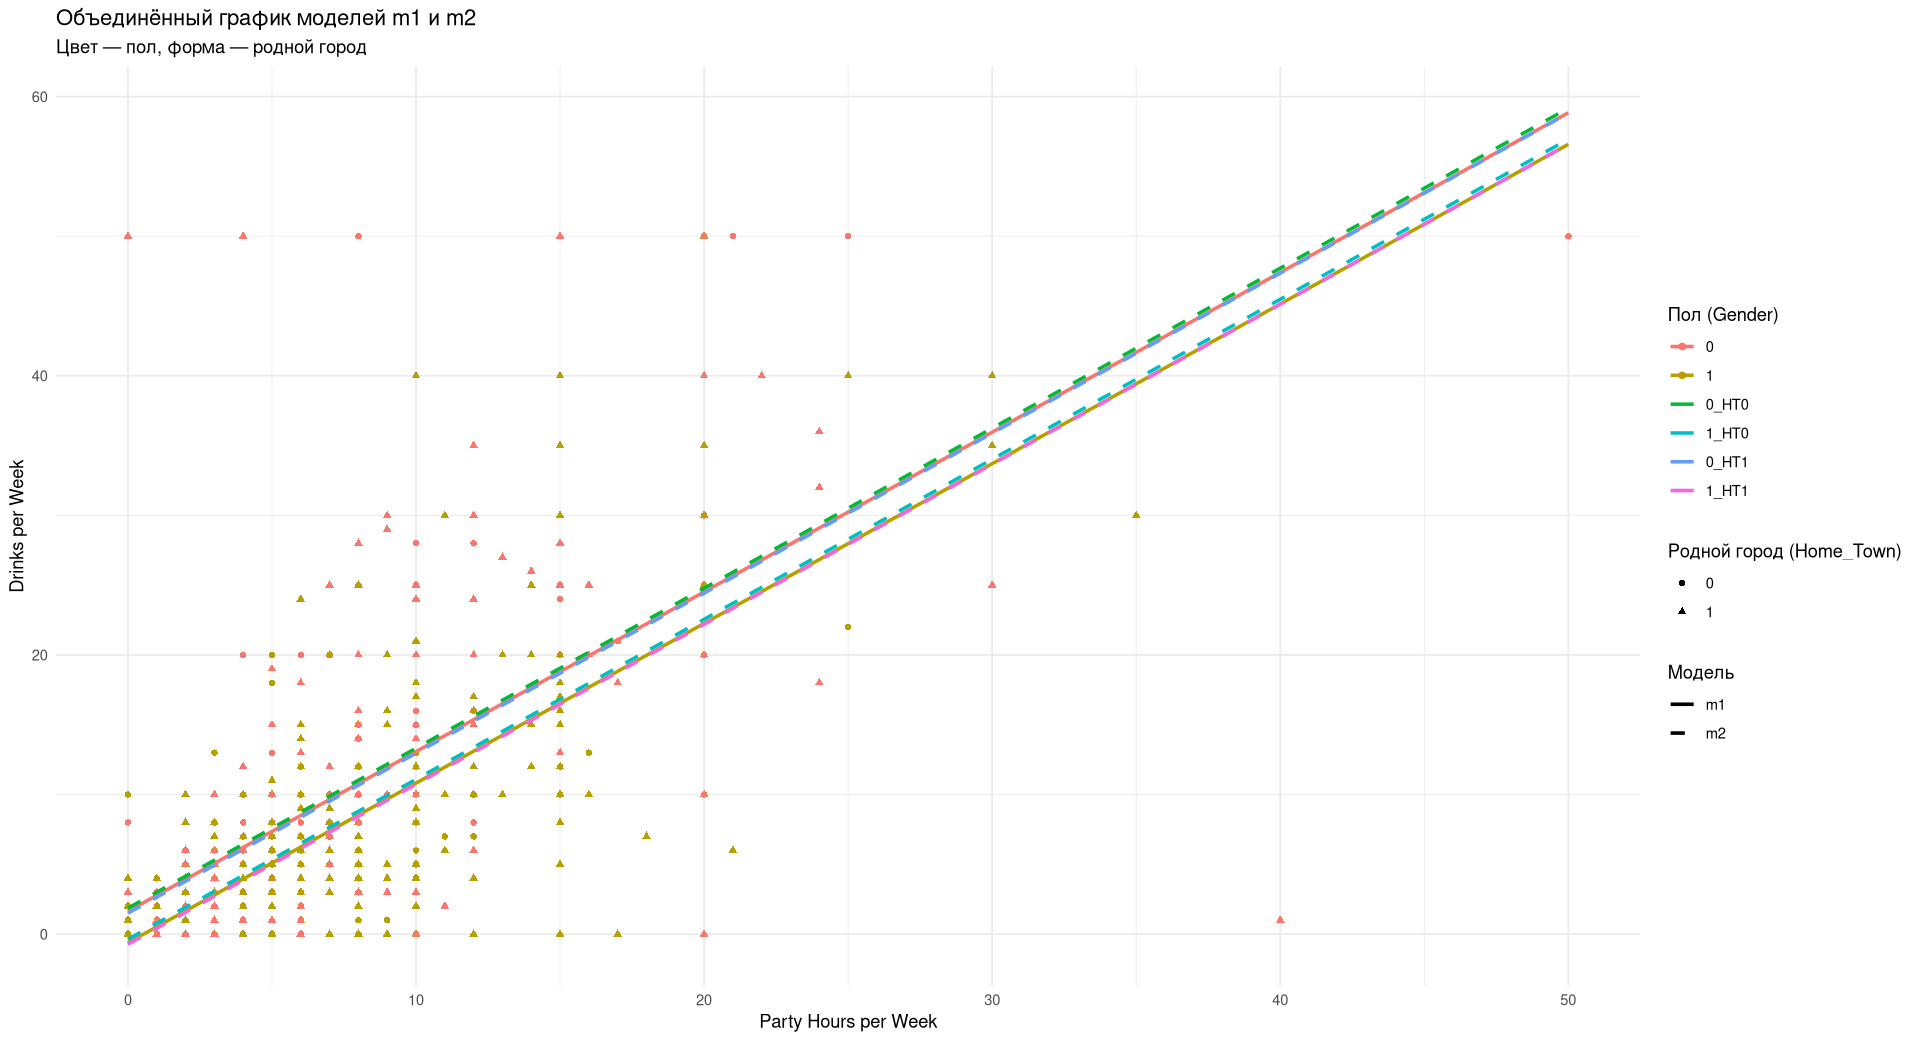
\includegraphics[height=0.6\textwidth]{imgs/models.png}  % Вставка изображения
	\caption{Графики моделей}  % Подпись к изображению
	\label{fig:models}  % Метка для ссылки
\end{figure}
Видно, что обе модели дают параллельные графики для каждого пола. Это связано с равенством коэффициента у переменной  Party\_Hours\_per\_week.
\newpage

Сделаем предсказание на +5\%, +10\% и +15\% от максимума по переменной вечеринок для обоих полов для первой модели. И создадим доверительный и предиктивный интервалы (рис. \ref{fig:intervals}).
\begin{figure}[h]  % Окружение для картинки
	\centering
	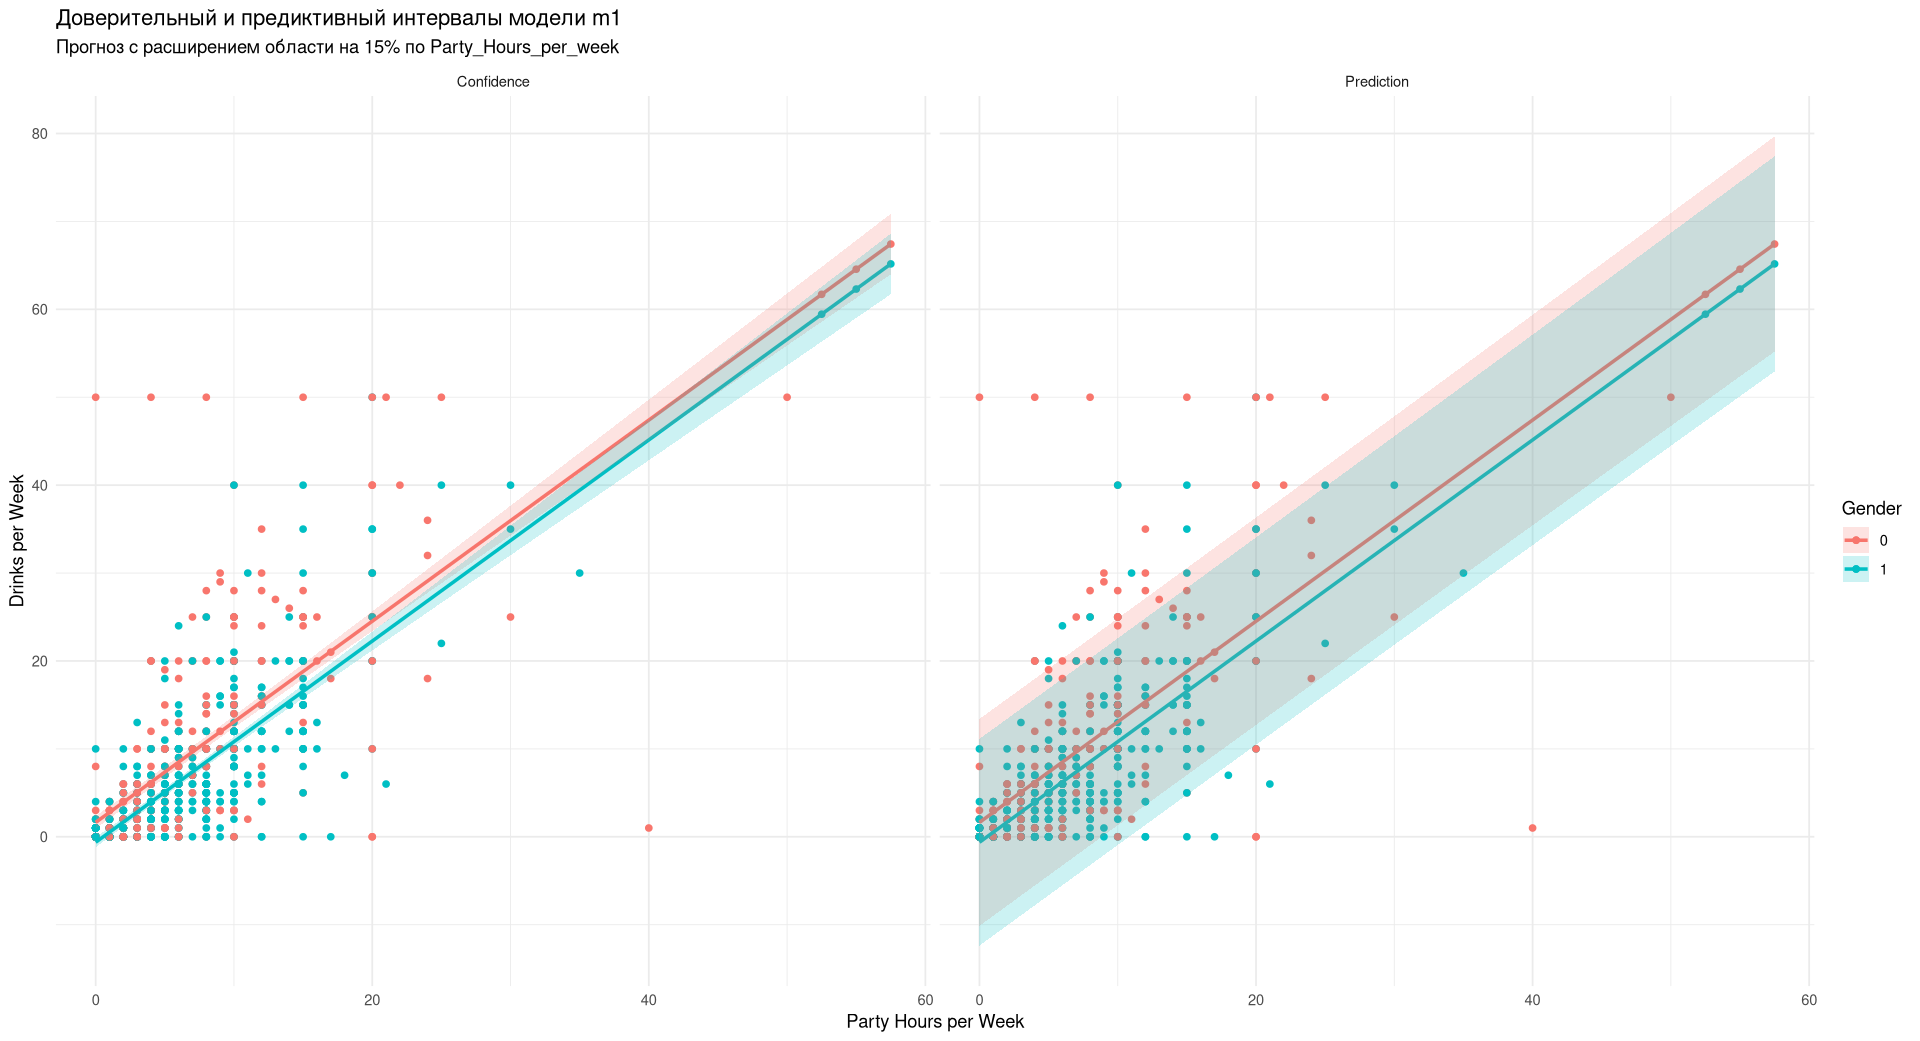
\includegraphics[height=0.6\textwidth]{imgs/intervals.png}  % Вставка изображения
	\caption{Графики интервалов моделей}  % Подпись к изображению
	\label{fig:intervals}  % Метка для ссылки
\end{figure}

